\documentclass[a4paper,12pt]{article}

\usepackage[utf8]{inputenc}
\usepackage{fontspec}
\usepackage{graphicx}
\usepackage{setspace}
\usepackage{pdfpages} 

\setlength{\parindent}{0pt}
\setlength{\parskip}{6pt}
%\setlength{\voffset}{-0.75in}

\setmainfont[
BoldFont=arialbd.ttf,
ItalicFont=ariali.ttf,
BoldItalicFont=arialbi.ttf
]{arial.ttf}

\author{Arundathi Shaji Shanthini}



\begin{document}
%%%%%%%%%%%COVERSHEET%%%%%%%%%%%%%%%%%
\begin{titlepage}
    \setlength{\voffset}{-1.6in}
    \noindent \noindent \makebox[\textwidth]{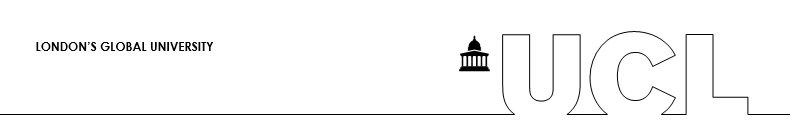
\includegraphics[width=1.55\textwidth]{files/Coversheet_Header.png}}
    
    \vspace{15mm}
    
    \begin{center}
        {\LARGE \textbf{BEng Project}}\\
        \vspace{4mm}
        {\Huge \textbf{Poster Presentation and Viva}}
    \end{center}
    
    \vspace{10mm}
    
    \begin{center}
    \begin{spacing}{1.8}
    {\LARGE
    Dynamic Modelling and Control of a Cable-driven Hyper-redundant Manipulator}
    \end{spacing}
    \end{center}
    
    \vspace{18mm}
    
     \begin{tabular}{ll}
    	\textbf{Student Name:}  & \hspace{4mm} Arundathi Shaji Shanthini \\
    	\textbf{Contact e-mail:} & \hspace{4mm} arundathi.shanthini.16@ucl.ac.uk \\
    	\textbf{Student number:} & \hspace{4mm} 16018351 \\ \\ 
    	\textbf{Project Supervisor:}  & \hspace{4mm} Prof. Sarah Spurgeon \\
    	\textbf{Contact e-mail:}  & \hspace{4mm} s.spurgeon@ucl.ac.uk \\
    	\textbf{Department:} & \hspace{4mm} Department of Electronic and Electrical Engineering\\ \\ 
    	\textbf{Submission Date:} & \hspace{4mm} 18\textsuperscript{th} of March 2020
    \end{tabular}
\end{titlepage}
%%%%%%%%%%%%%%%%%%%%%%%%%%%%%%%%%%%%%%

\pagebreak

\section{Presentation Transcript}
Robotic manipulators that mimic the motion of snakes are highly desired for the high manoeuvrability and accessibility properties that they offer. Such a robotic arm developed by OC Robotics has been made available at Here East in an attempt to automate close range measurements and inspection of aerodynamic structures using cutting edge imaging techniques like photogrammetry (research of which is undertaken by a group called 3DIMPact of UCL CEGE). Since this robot was commissioned, many applications of this robotic arm were realised, one of which was also close-range inspection of aerodynamic surfaces to understand structural defaults. However, controlling the end-effector position and automating this process has been a challenge given that currently the robot’s control is facilitated via a proprietary software provided by OC Robotics. Therefore, a control strategy that facilitates precise control of the robot needed to be developed. My project aims to contribute to this modelling and control research effort undertaken by the UCL Institute of Robotics. The main objective of the project is to simulate the robotic arm and design a control strategy for the same using Simulink. Further, it also briefly looks into the robustness of the control strategy that was developed. 

What makes the project work novel is that simulation of cable-driven hyper-redundant manipulator (CDHRM) using its dynamic model hasn’t been done so far. Literature review suggests that all the control effort associated to CDHRM and systems similar to it have been performed on the actual robot so this meant that dynamic model of the CDHRM as such has not been studied in detail yet.

The cable-driven hyper-redundant manipulator (CDHRM) is a hollow core structure with passive universal joints between each link (facilitating pitch-yaw motion). Each joint is driven by wire ropes that are controlled by motors at the base. This video shows the exact robot at Here East. Each link is controlled by 3 cables placed equidistant to each other around the link. The nose (the last link) of the snake arm can be used to attach different payloads (measuring equipment, camera, manipulator claws etc.) and the hollow core facilitates any cables that may be required by the payload at the end of the arm for power and communication. This is in fact one of the major advantages of this structure, all the electronics including the actuators, control hardware etc. are at the base of the robot which means that this robot can function even in hazardous conditions.

The control objective here is to obtain very low error (within  0.1mm tolerance) in the tracking of end-effector position. However, this is challenging because the end-effector position can only be indirectly controlled by the cables that are attached to the actuator (motors) whose angle of rotation can be controlled. This immediately makes us understand that to obtain the reference value in amount of angle of rotation of motor we need to understand the kinematic model of the system in order to derive this value from the desired end-effector position. As can be seen in the diagram, (under section – Modelling the system) this requires mapping between different spaces. Each space describes a set of equations that converts from one measure to the other. The forward kinematics can be mapped as angle of rotation of motors → change in length of cable → joint angles (shape of the robot arm) → end-effector position. 

The dynamic model of the system can be thought of as similar to that of a normal robotic manipulator with passive universal joints so the equation used is similar to that of a generic robotic manipulator (refer equation in the section – Modelling the system) where the input torque (τ on the RHS is usually the torque due to the motors in between 2 links) is replaced by torque acting on the link due to the cables. Equations involving the cable dynamics (input to the dynamic block) is derived using a Newton-Euler recursive approach.

The control configuration involves using a feedback plus feedforward strategy with a PID controller. Figure 2 is a screenshot from its implementation in Simulink. The purple area in the figure is the reference input – the end-effector position. The pink area contains all the blocks implementing the inverse kinematics. The output at the end of this gives the reference value of angle of rotation of the motor. This signal is then used as input into a feedback plus feedforward control configuration. The output of this (manipulated variable) is then input to the dynamic block representing the arm (the plant). The output of the plant is then converted back to end-effector position using forward kinematic relationship that converts the signal from joint space to task space. This is then used to calculate the error in tracking the reference value of end-effector position (value observed by the scope). As evident the error of the end effector position is not being used in the feedback to the controller this is probably something to note for the future to develop even better control configurations.

Under Preliminary Results section, what I have shown is the tracking results I obtained on modelling the actuator of the snake arm. The actuator was identified as a maxon motor so equation from its datasheet was used to derive the model of the motor. This was the progress as on 10th of March and progress has been made since on the actual simulation itself. A part of the project also involved analysing the robustness of the model this is to be done by changing end-effector mass (Ftip on the RHS of the dynamic model) and by introducing an extra term for external forces (Fext) on the RHS. Changes to these values will be used to analyse the changes to the tracking error of the end-effector position.

As I talked through the aims and objectives of my project and work undertaken it might be understood that while I have performed the simulation of this system using what I think is a good dynamic model future work must be undertaken to verify and validate the behaviour and performance of the dynamic model. The project aimed to be the first stepping stone towards achieving the bigger goal of implementing and achieving precise control of the robotic arm. Another approach to model the robot could also have been to use tools like Simscape to record values from the actual robot and obtain an approximate model from the software itself. One of the limitations of the current simulation so far is that all parameters that are being used currently, are just dummy values for the purpose of simulation. Even otherwise, it is known that error in dynamic parameter estimation affects the results of the simulation. So, using existing methods to reduce the error that this adds to simulation can help improve the simulation of results as well. Finally, when a satisfactory reliable simulation is developed, future work would also involve implementation of the control strategy on the actual robot and evaluating its performance.

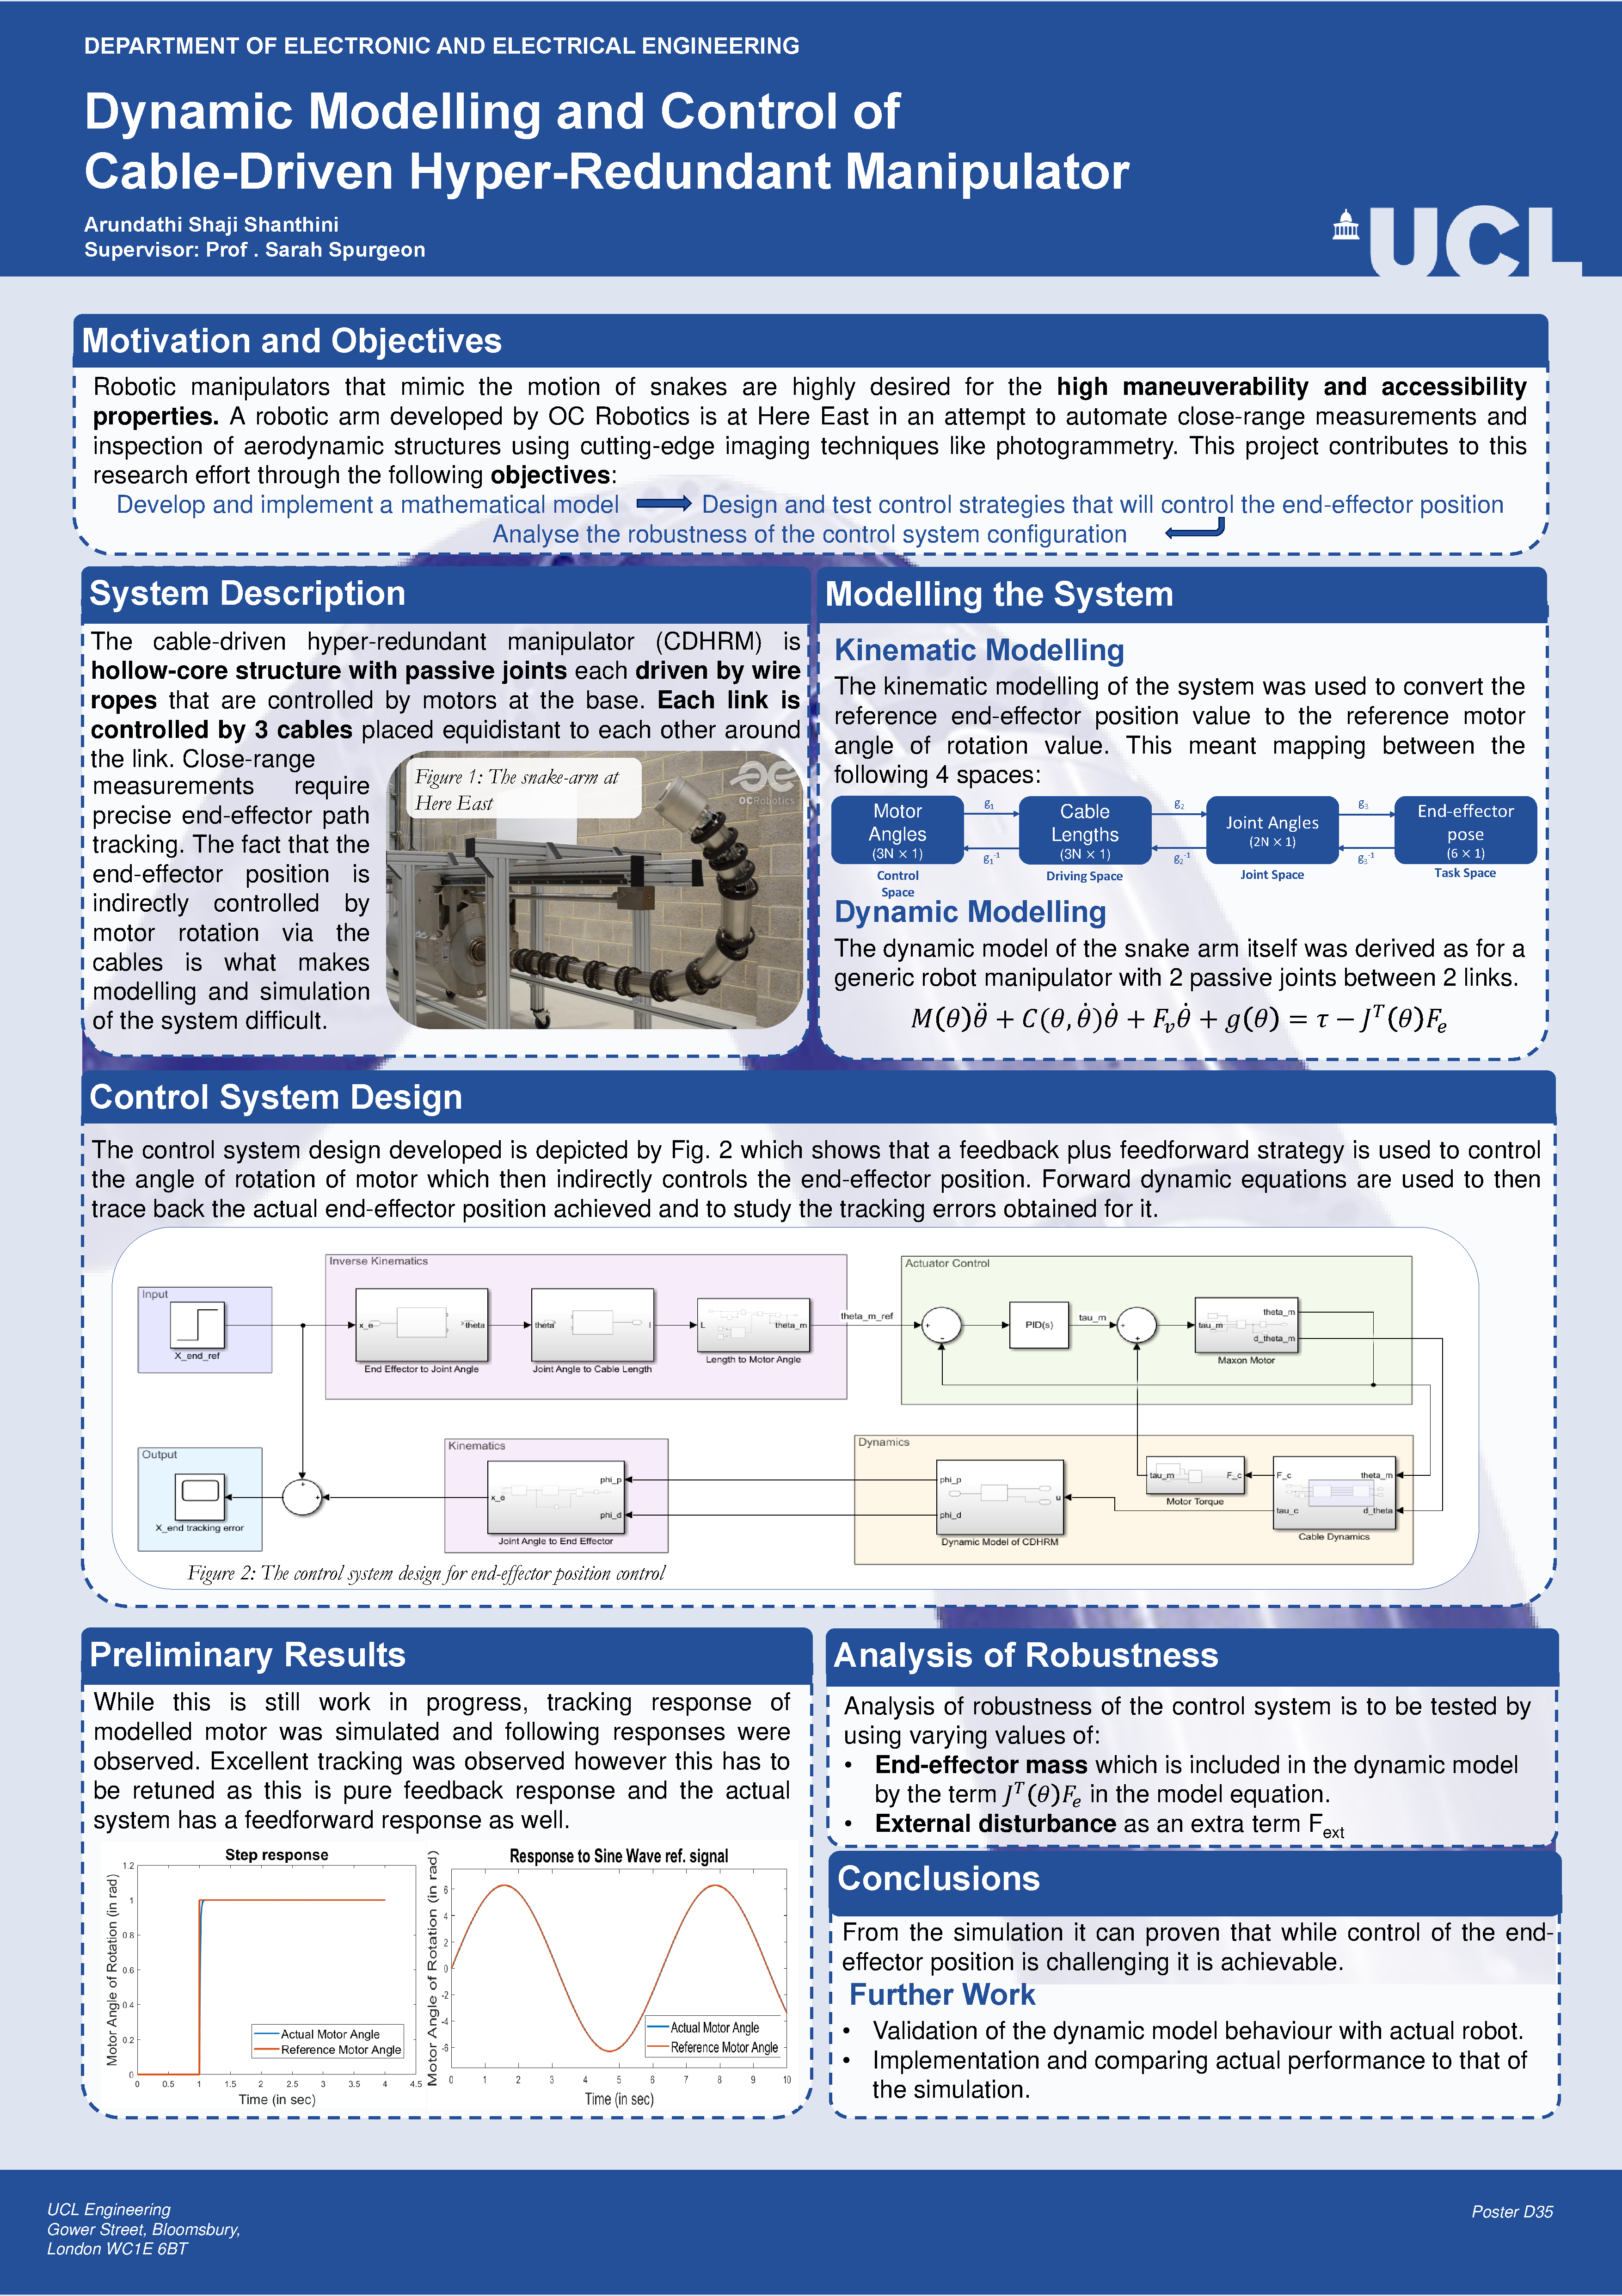
\includepdf[page=-]{files/Poster - D35 - Arundathi Shaji - A1}
\section{Answers to Viva Questions}
\textbf{What motivates you to involve feed-forward control?}

Feedforward control is usually adopted to compensate/eliminate any effect of measurable disturbances even when there are modelling errors. It is known that a combined feedback plus feedforward control can significantly improve the performance of the control system in comparison to a feedback only control especially in cases where these disturbances can be measured or modelled. 

Usually the decision of whether or not to involve a feedforward control is governed by the degree of improvement this provides when added to the design. It is the results stated in \cite{RN30} from the experiments on a physical CDHRM system that motivated me to involve a feedforward control. In this paper, they provide evidence of how using a feedback plus feedforward approach improved the results in controlling the CDHRM. They have stated the maximum error in end-effector position control observed when using feedback only control is 20mm. On introducing feedforward control to it this decreased to 2mm.

\hspace{10pt}

\textbf{Are you the first one to attempt to develop a mathematical model for the system in Fig. 1 (poster)? If not, how does your model compare to other work?}

From my literature review, my understanding is that mathematical modelling and simulation of a similar system has not been done in the past. All papers I could find perform experiments on the actual robot itself and none involves simulation of this kind of robotic manipulator. While the kinematic model of the CDHRM (the system shown in Figure 1) has been already studied very well. I believe the study of its dynamics is still novel. \cite{RN30} is the only source I found that discusses the dynamics of a CDHRM (just the cable dynamics) and this paper was published in 2018.

While working on it I realised that the dynamic model of this robot can be represented by the standard dynamic model equation of a generic robotic manipulator (the equation under section – Modelling the system in the poster) because this robot is exactly similar to that of any normal robotic manipulator except that all its joints are passive and the torque due to the driving cables can be considered as the input signal. The equation in the poster is a standard in robotics for modelling robotic systems and what I did was, calculate those terms based on the parameters and structure of the given CDHRM which I believe represents the behaviour of the system itself. However, validating the behaviour of the model using data from the actual system remains as future work to be undertaken.

\hspace{10pt}

\textbf{The results are very preliminary. How do you expect your model to work with real-world signals?}

Yes the results in the poster are very preliminary, and this was as per the progress around the beginning of March at which point I had only all the individual blocks (Kinematic Model and Dynamic Model) working separately. My approach was to individually test each block and validate it to ensure that they behave as expected before I would combine them together. The Screenshot from Simulink (Figure 2) is the final implementation and results from those (I am currently working on tuning them) haven’t been obtained yet. 

The expected input signal will be set a way points for the robot. In the real implementation this will come from a path planner algorithm which will also ensure that the waypoints are within the task space of the robot. However, implementing this is currently beyond scope of this project. Usually, if the controller performs well with these simple test signals (test signals will include both planar waypoints and spatial waypoints) then it would also map well with other signals. The signals are expected to be either straight lines along a plane (for scanning) or going to pre-defined points in steps (for imaging) so the real-world signals should be similar to these test signals. However, testing these with difficult input signals would definitely be work for the future to test the limits of its performance upon implementation.

\pagebreak
\bibliographystyle{IEEEtran}
\bibliography{references}
\end{document}